\documentclass[12pt]{report}
\usepackage[margin=1in]{geometry}
\usepackage{hyperref}
\usepackage{url}
\usepackage{xurl}
\hypersetup{breaklinks=true}
\usepackage{graphicx}
\usepackage{amsmath}
\usepackage{enumitem}
\usepackage{float}

\title{Week 6 Report}
\author{Dhanush Balusa}
\date{June 25, 2025}

\begin{document}

\maketitle

\chapter*{Research}

\noindent \textbf{Consequence of a Collision:}
\begin{itemize}
  \item Reference: \url{https://ntrs.nasa.gov/api/citations/19910011417/downloads/19910011417.pdf}
  \item Focuses on the lack of data regarding small debris (1mm to 10cm) in low Earth orbit.
  \item Highlights that collisions are a significant source of debris, with no significant momentum transfer observed in breakup events.
  \item Proposes a two-component model for collisional breakups, distinguishing between directly and indirectly affected materials.
  \begin{itemize}
    \item Directly Affected Materials: These are the components that directly experience the impact and participate in the momentum transfer during the collision.
    \item Indirectly Affected Materials: These materials are not directly hit but are affected by the resulting shock waves and debris cloud, which can lead to larger fragments.
    \item In on-orbit tests, only the indirectly affected materials, which form a larger explosion-type debris cloud, have been observed, while momentum transfer is limited to the directly involved materials characterized by the column mass of the target.
  \end{itemize}
  \item Emphasizes the need to understand momentum transfer as frequency of collisions in space increases, particularly with the anticipated use of anti-satellite weapons, as it can significantly influence the amount and distribution of debris generated from such events.
  \item Concludes that accounting for momentum transfer can reduce the amount of debris in long-life orbits; however, it currently overlooks the impact of relative velocity and requires further validation through hypervelocity impact tests.
\end{itemize}

\noindent \textbf{Break-up Model:}
\begin{itemize}
  \item Reference: \url{https://ntrs.nasa.gov/api/citations/20070007324/downloads/20070007324.pdf}
  \item The Fengyun-1C spacecraft was intentionally destroyed on January 11, 2007, creating over 2,000 pieces of debris.
  \item The breakup event was caused by a kinetic anti-satellite test conducted by China, which involved a direct-ascent missile intercepting the satellite at a relative velocity of approximately 9 km/s (hypervelocity impact).
  \item The U.S. Space Surveillance Network tracked the debris, revealing long-lived orbits and significant risks to operational spacecraft.
  \item The event marked the worst single fragmentation in space history, increasing the LEO debris population by over one-third.
  
  \begin{figure}[H]
    \centering
    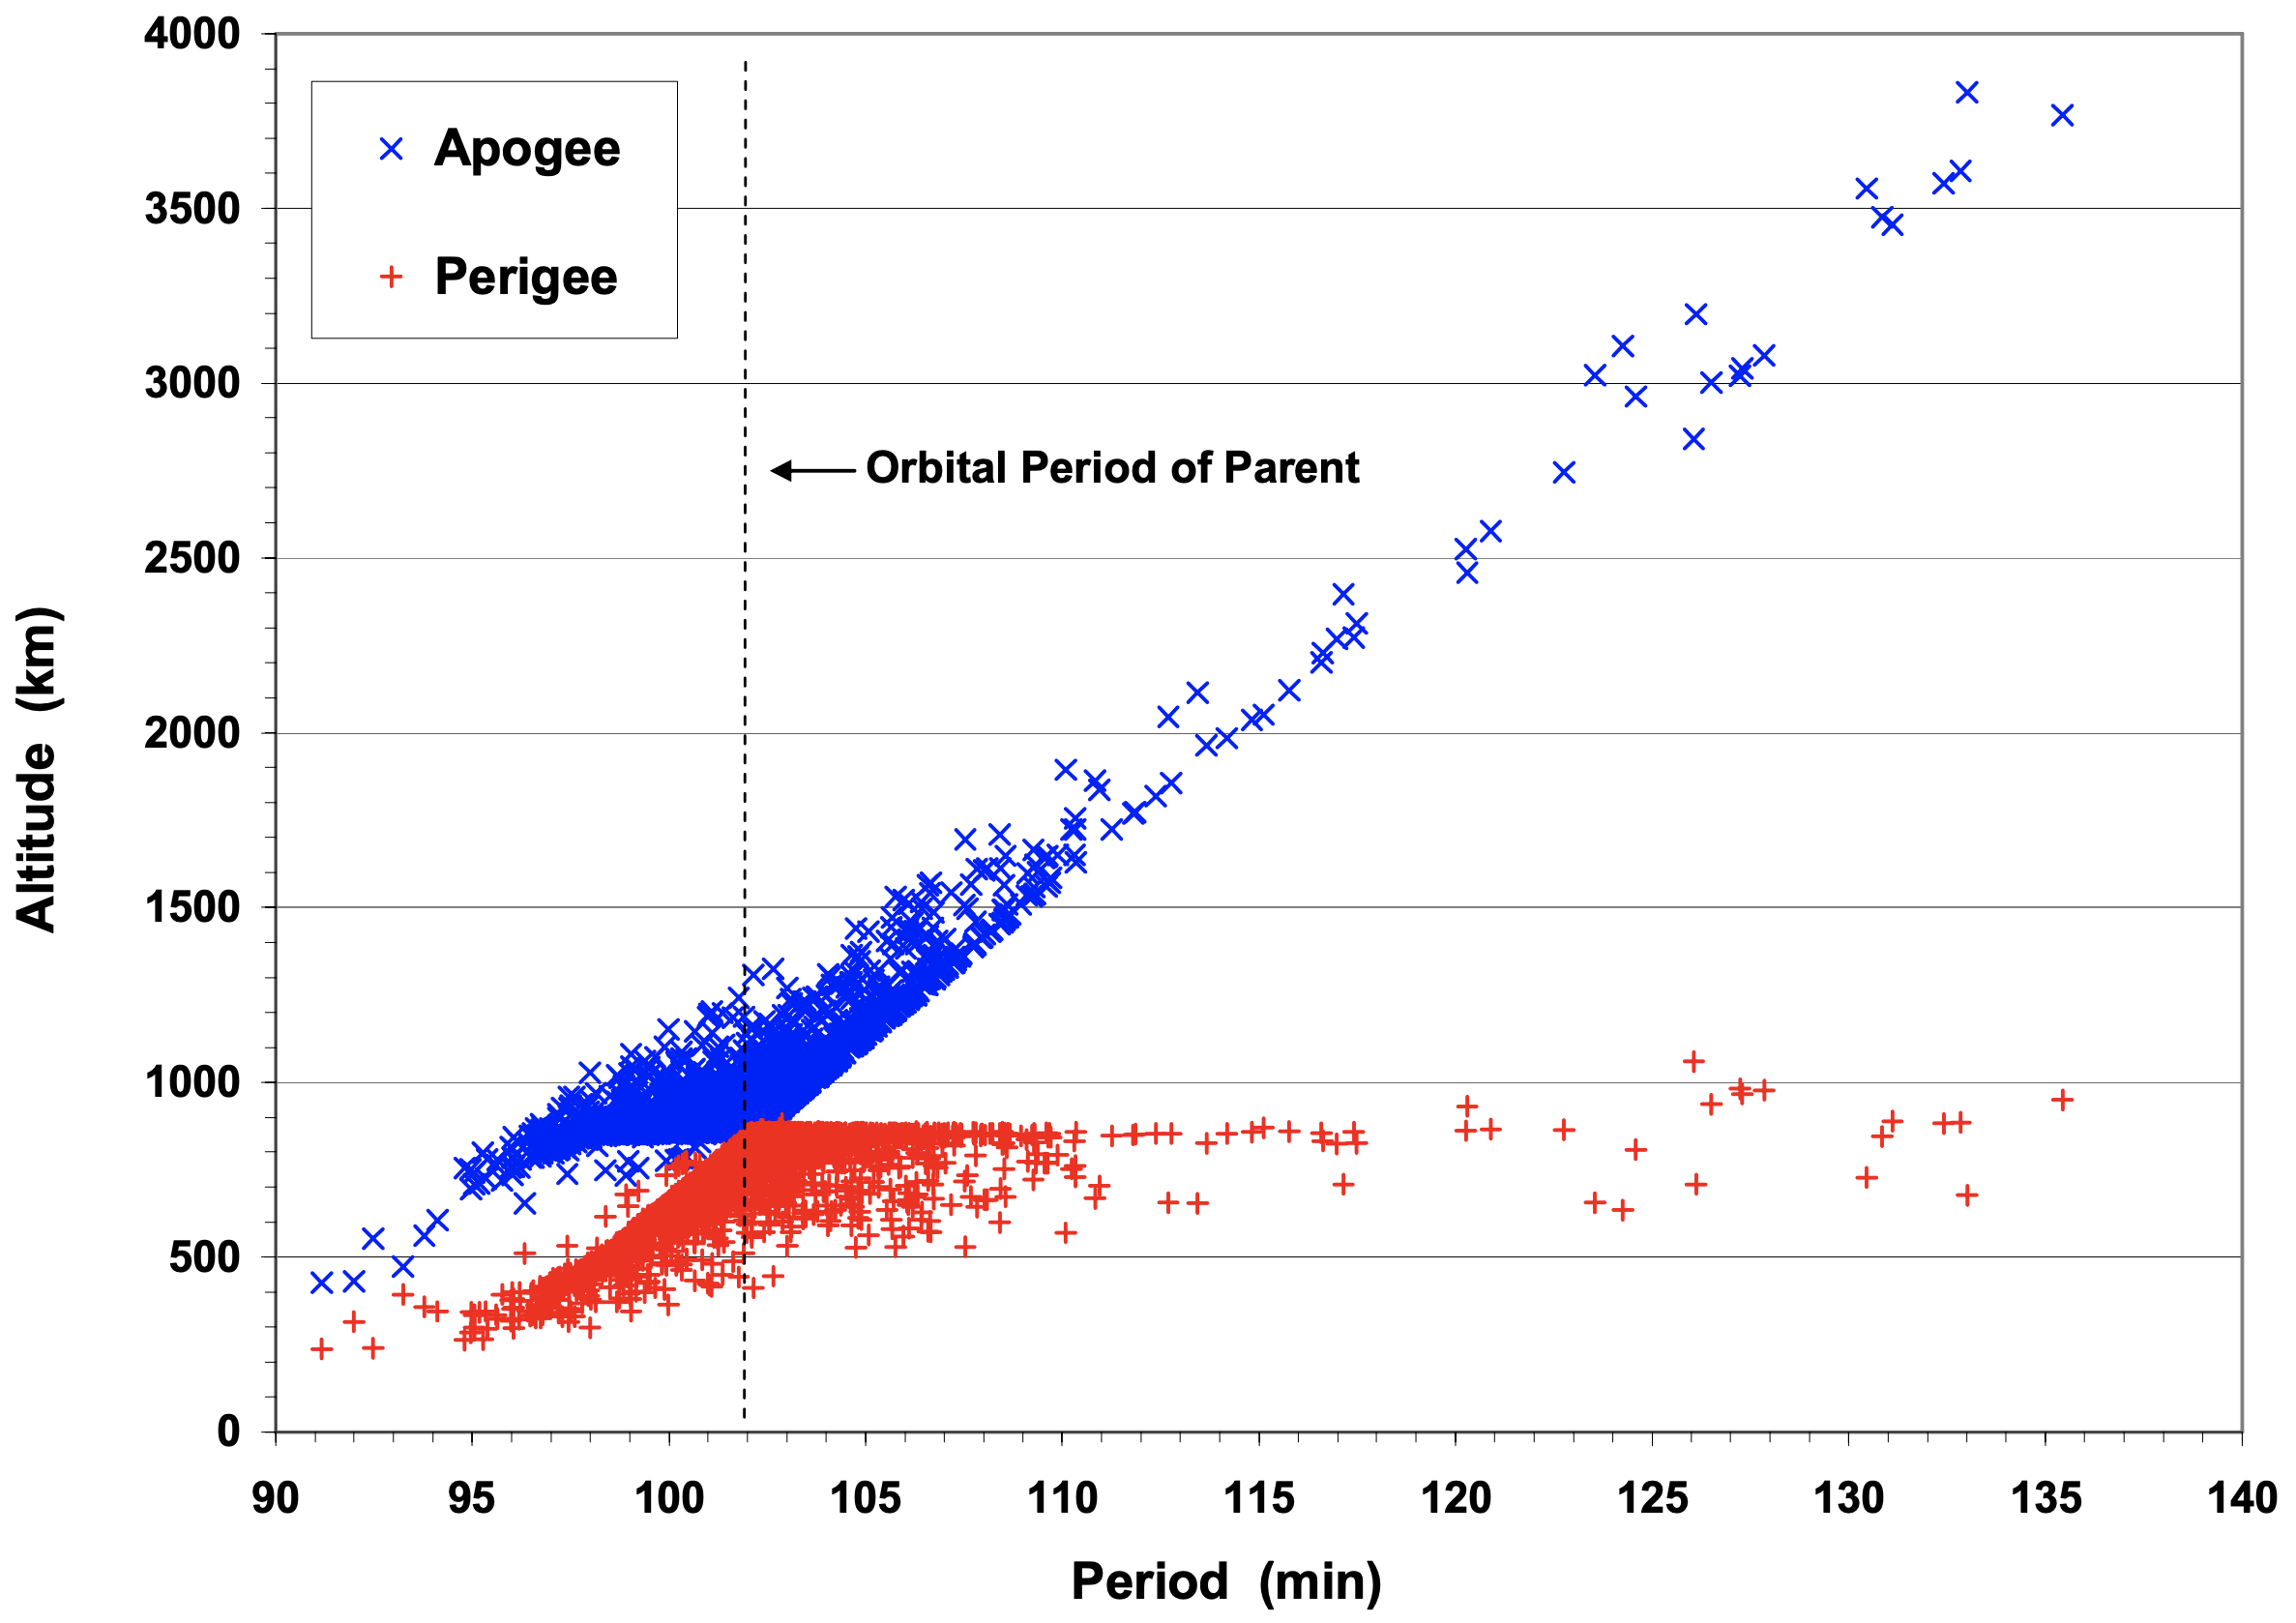
\includegraphics[width=0.8\textwidth]{figure_week_6_gabbard-diagram.png}
    \caption{A Gabbard diagram (apogee and perigee versus orbital period) of the Fengyun-1C orbital debris cloud as assessed on 11 July 2007, six months after the break-up with a total of 2347 objects individually identified.}
    \label{fig:Gabbard diagram}
  \end{figure}
  
  \begin{figure}[H]
    \centering
    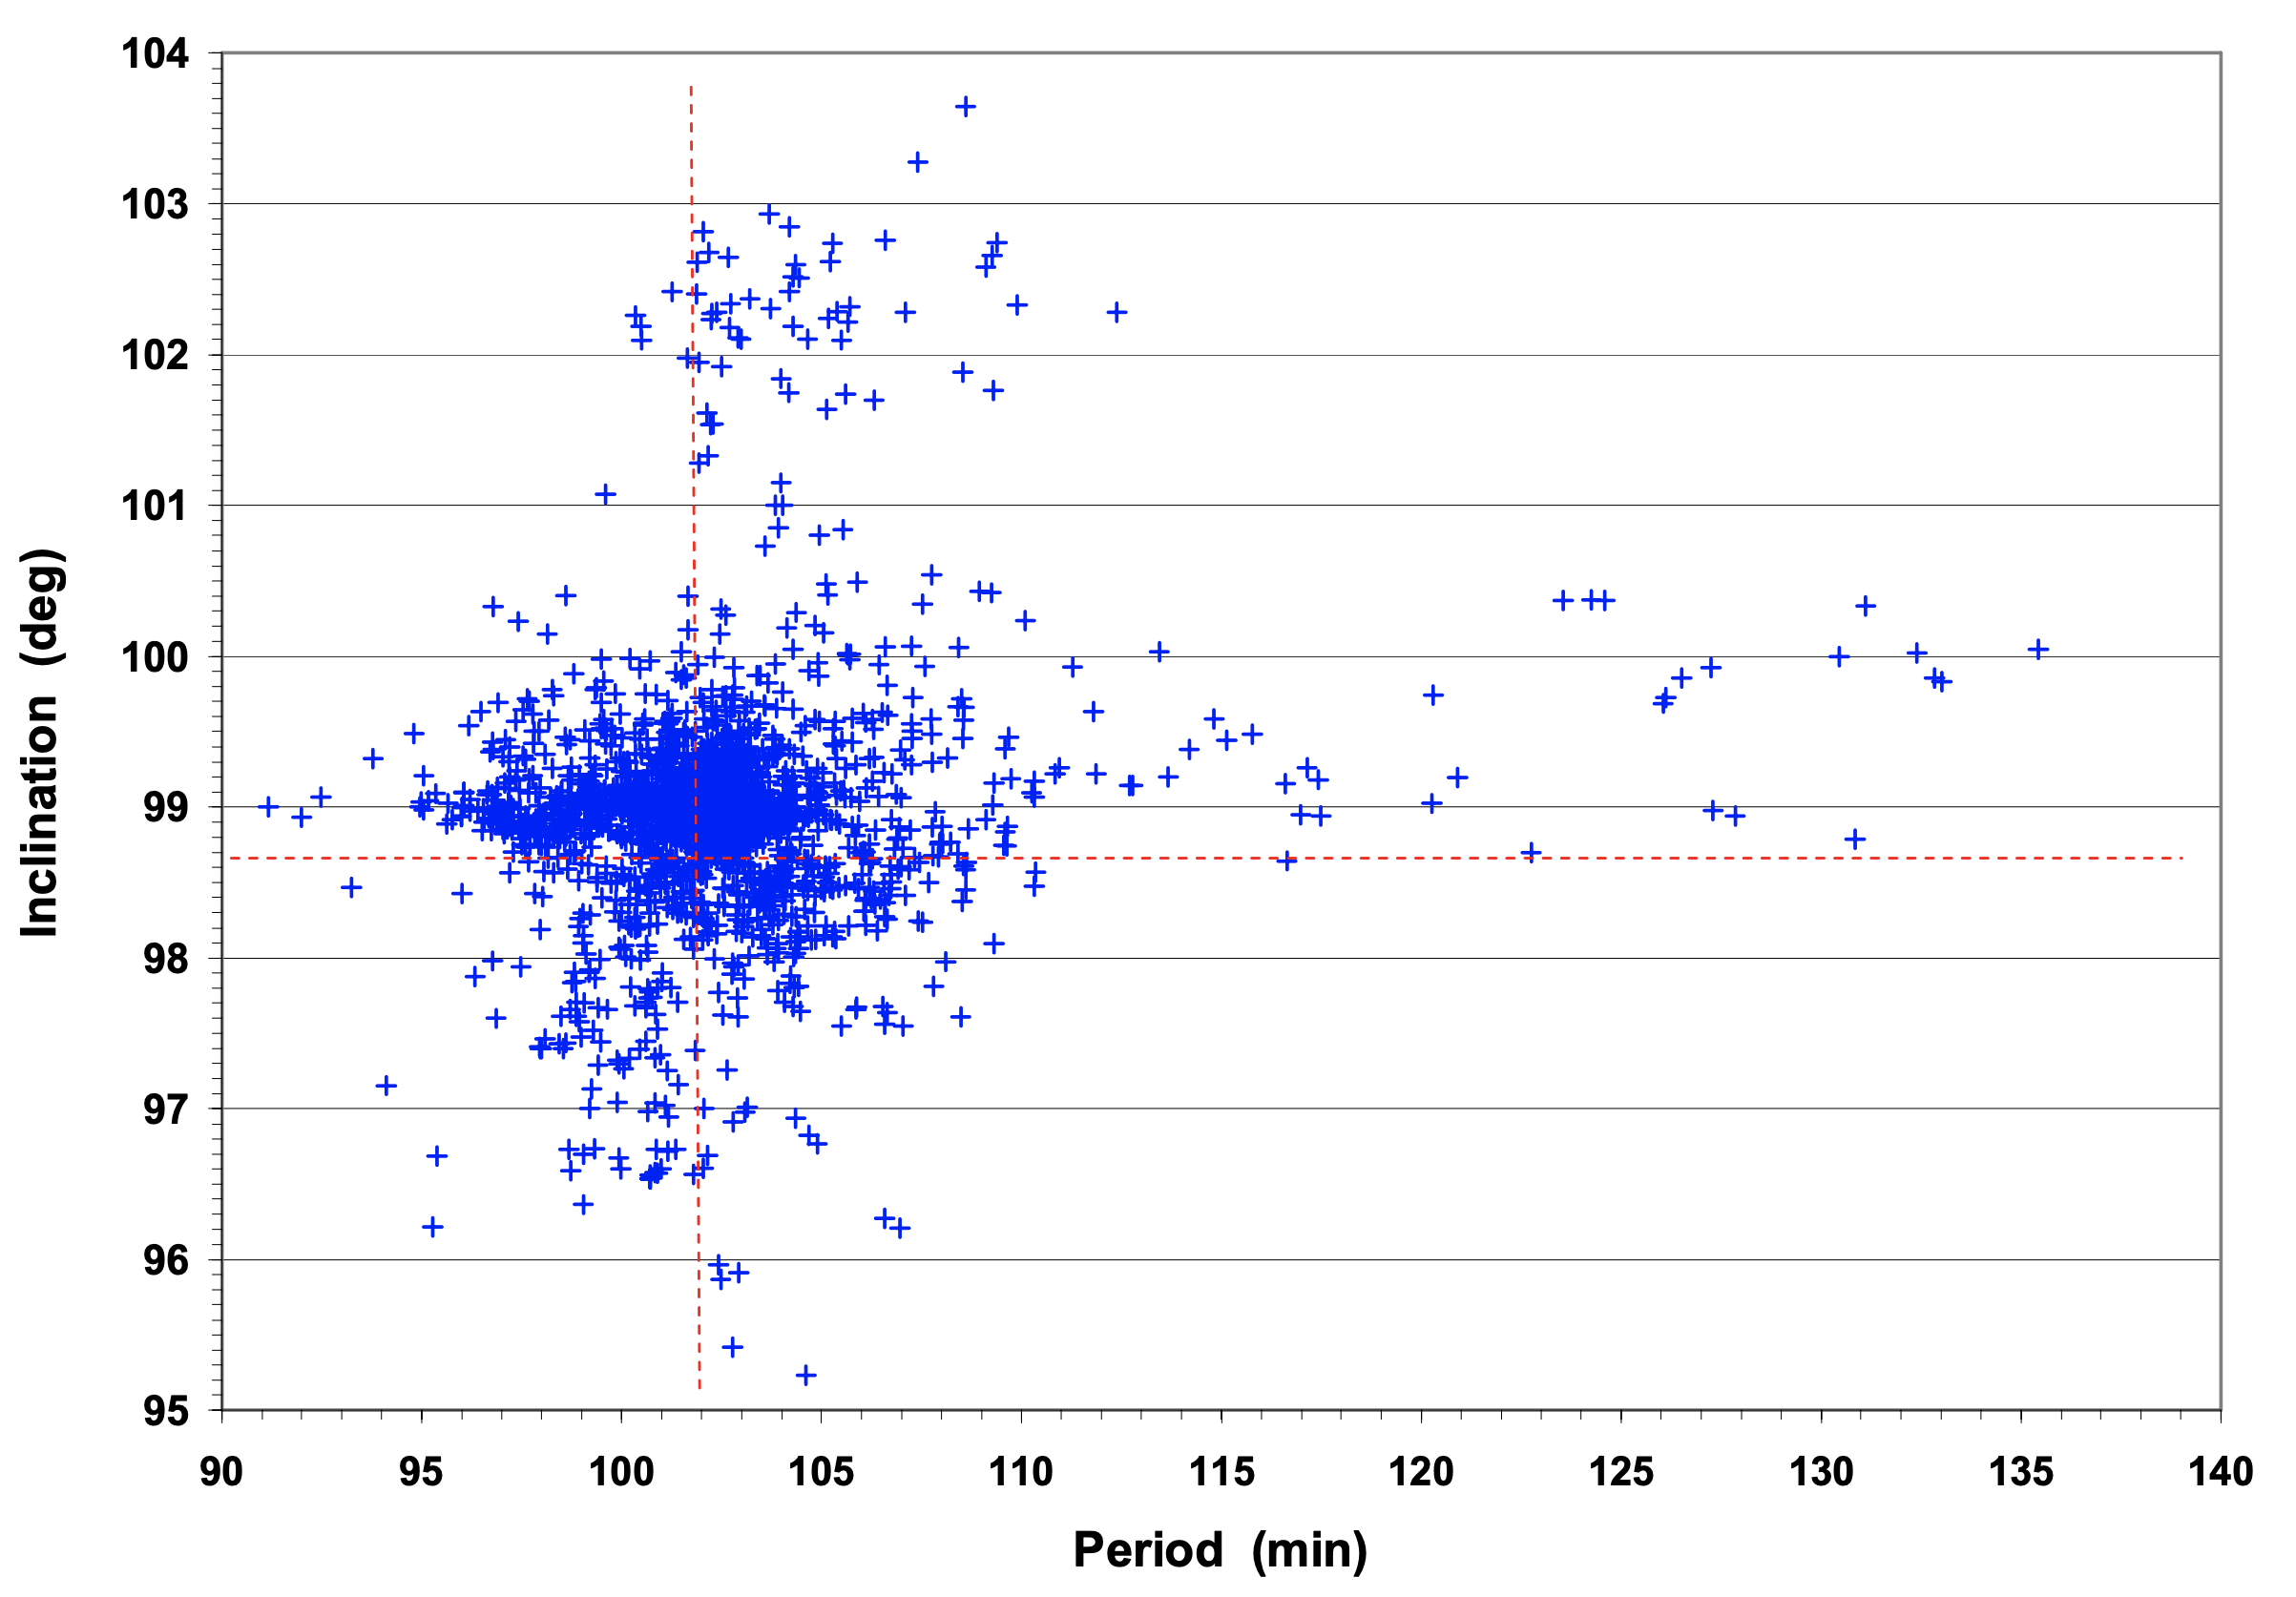
\includegraphics[width=0.8\textwidth]{figure_week_6_F-1C-inclination.png}
    \caption{Approximately 80\% of the tracked debris were found in inclinations greater than those of the spacecraft prior to impact.}
    \label{fig:F-1C inclination}
  \end{figure}

  \item The debris poses ongoing collision risks, with potential long-term environmental impacts in LEO.
  
  \begin{figure}[H]
    \centering
    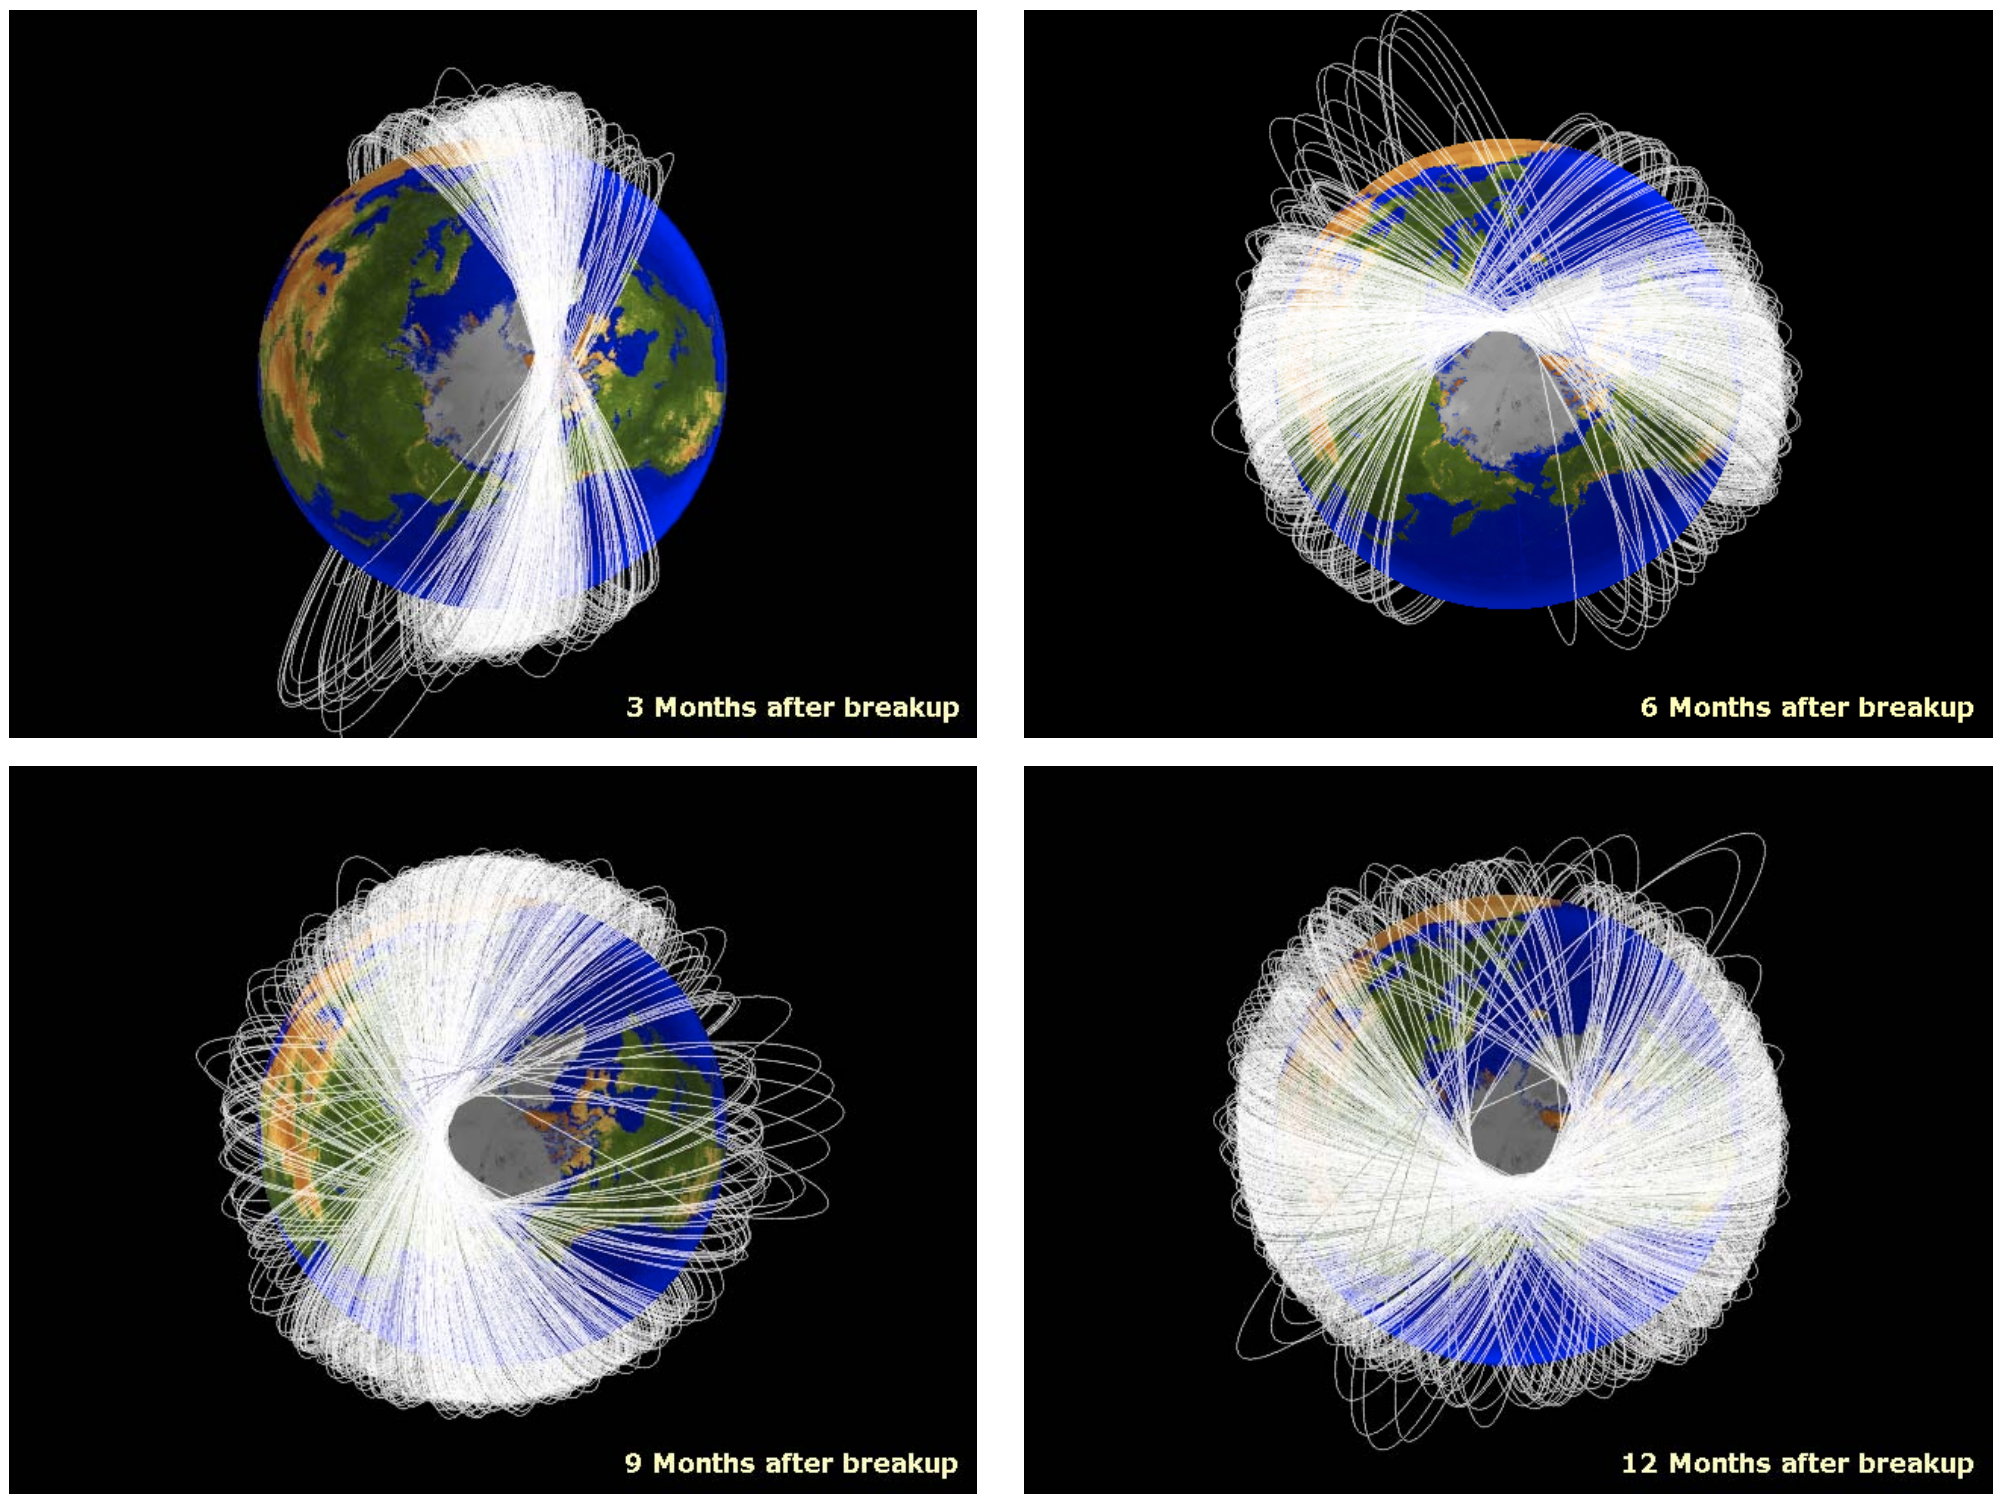
\includegraphics[width=0.8\textwidth]{figure_week_6_F-1C-orbit-evolution.png}
    \caption{Evolution of the Fengyun-1C debris orbit planes.}
    \label{fig:F-1C-orbit-evolution}
  \end{figure}

\end{itemize}

\noindent \textbf{Hypervelocity Impact:}
\begin{itemize}
  \item Reference: \url{https://www.esa.int/Space_Safety/Space_Debris/Hypervelocity_impacts_and_protecting_spacecraft}
  \item Hypervelocity Collisions: Defined as impacts with velocities $ \ge $ 4 km/s, common in LEO.
  \item Collision Types:
  \begin{itemize}
    \item Catastrophic: Both target and impactor destroyed.
    \item Non-Catastrophic: Impactor destroyed, target damaged.
  \end{itemize}
  \item Fragment Distribution: More small fragments produced than large; modeled using empirical formulas.
  \item Orbital Changes: Fragments assume new orbits based on ejection velocity; Gabbard diagrams illustrate orbital decay and distribution.
  
  \begin{figure}[H]
    \centering
    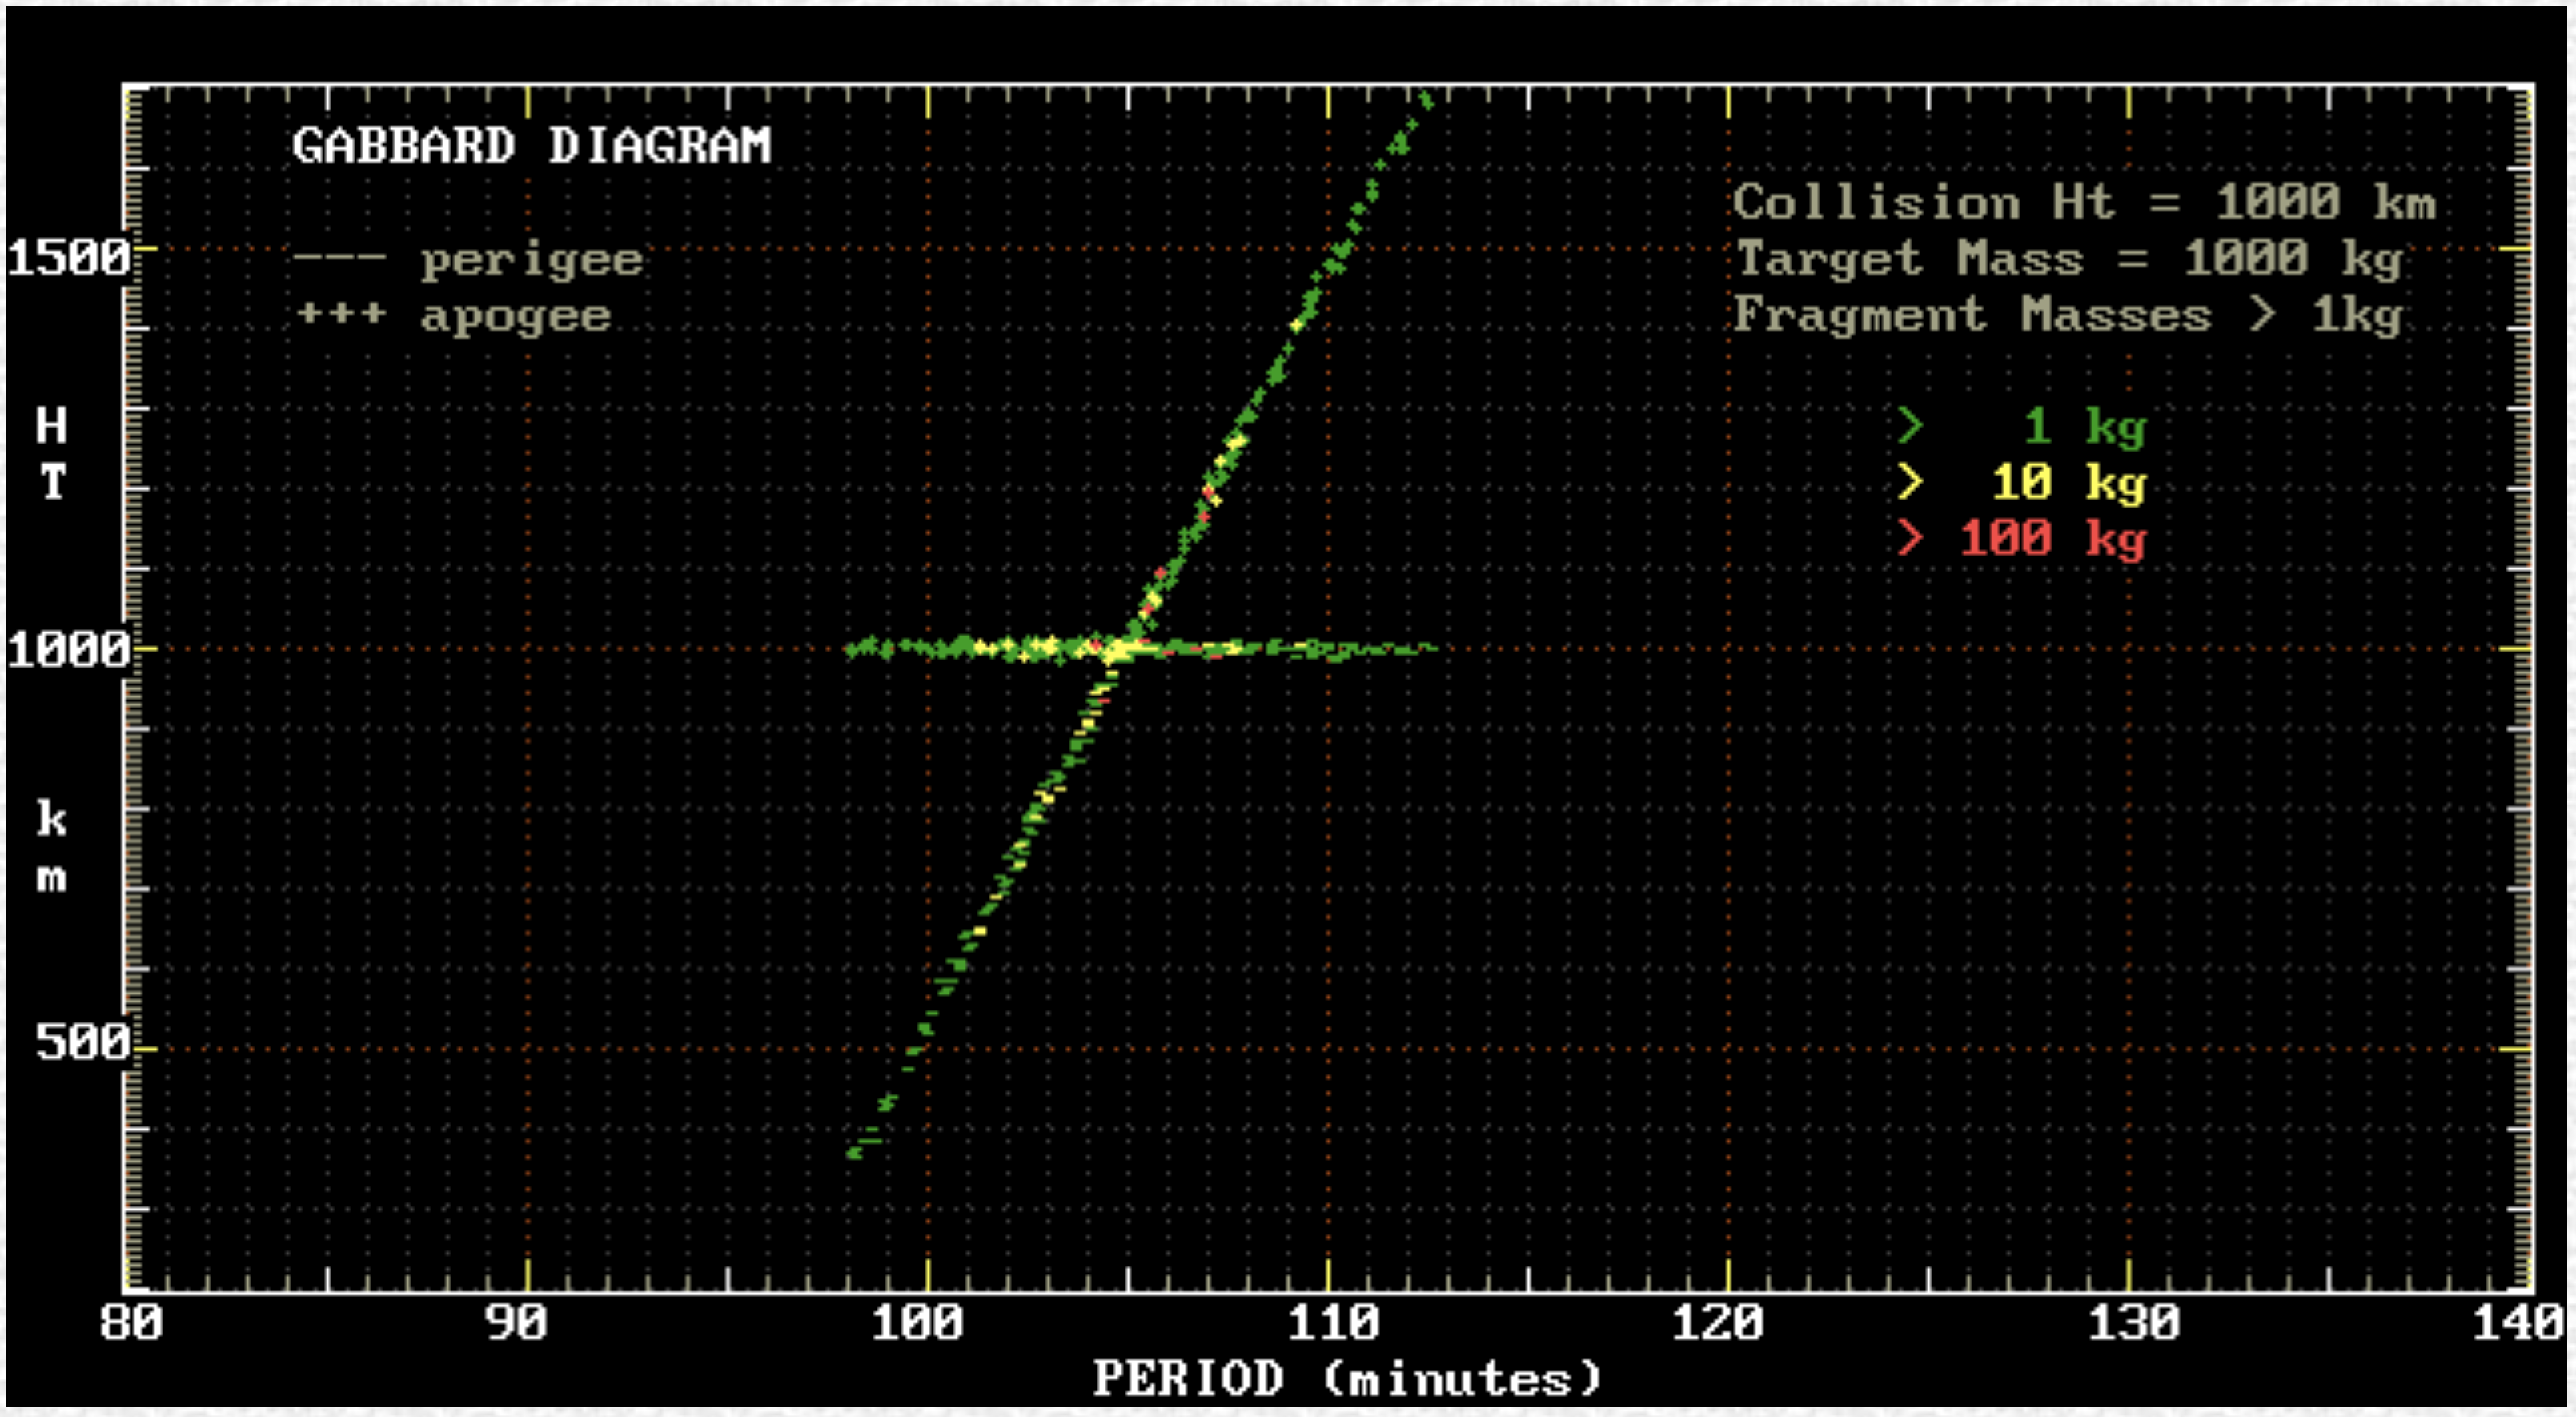
\includegraphics[width=0.8\textwidth]{figure_week_6_gabbard-diagram-au.png}
    \caption{It can be seen that the largest masses ($ \ge $ 100 kg) are relatively close to the original orbit, whereas the smallest masses ($ \ge $ 1kg) are the most dispersed.}
    \label{fig:gabbard-diagram-au}
  \end{figure}

  \item Debris Behavior: Smaller fragments burn up upon re-entry; larger fragments decay slower due to atmospheric drag.
  
  \begin{figure}[H]
    \centering
    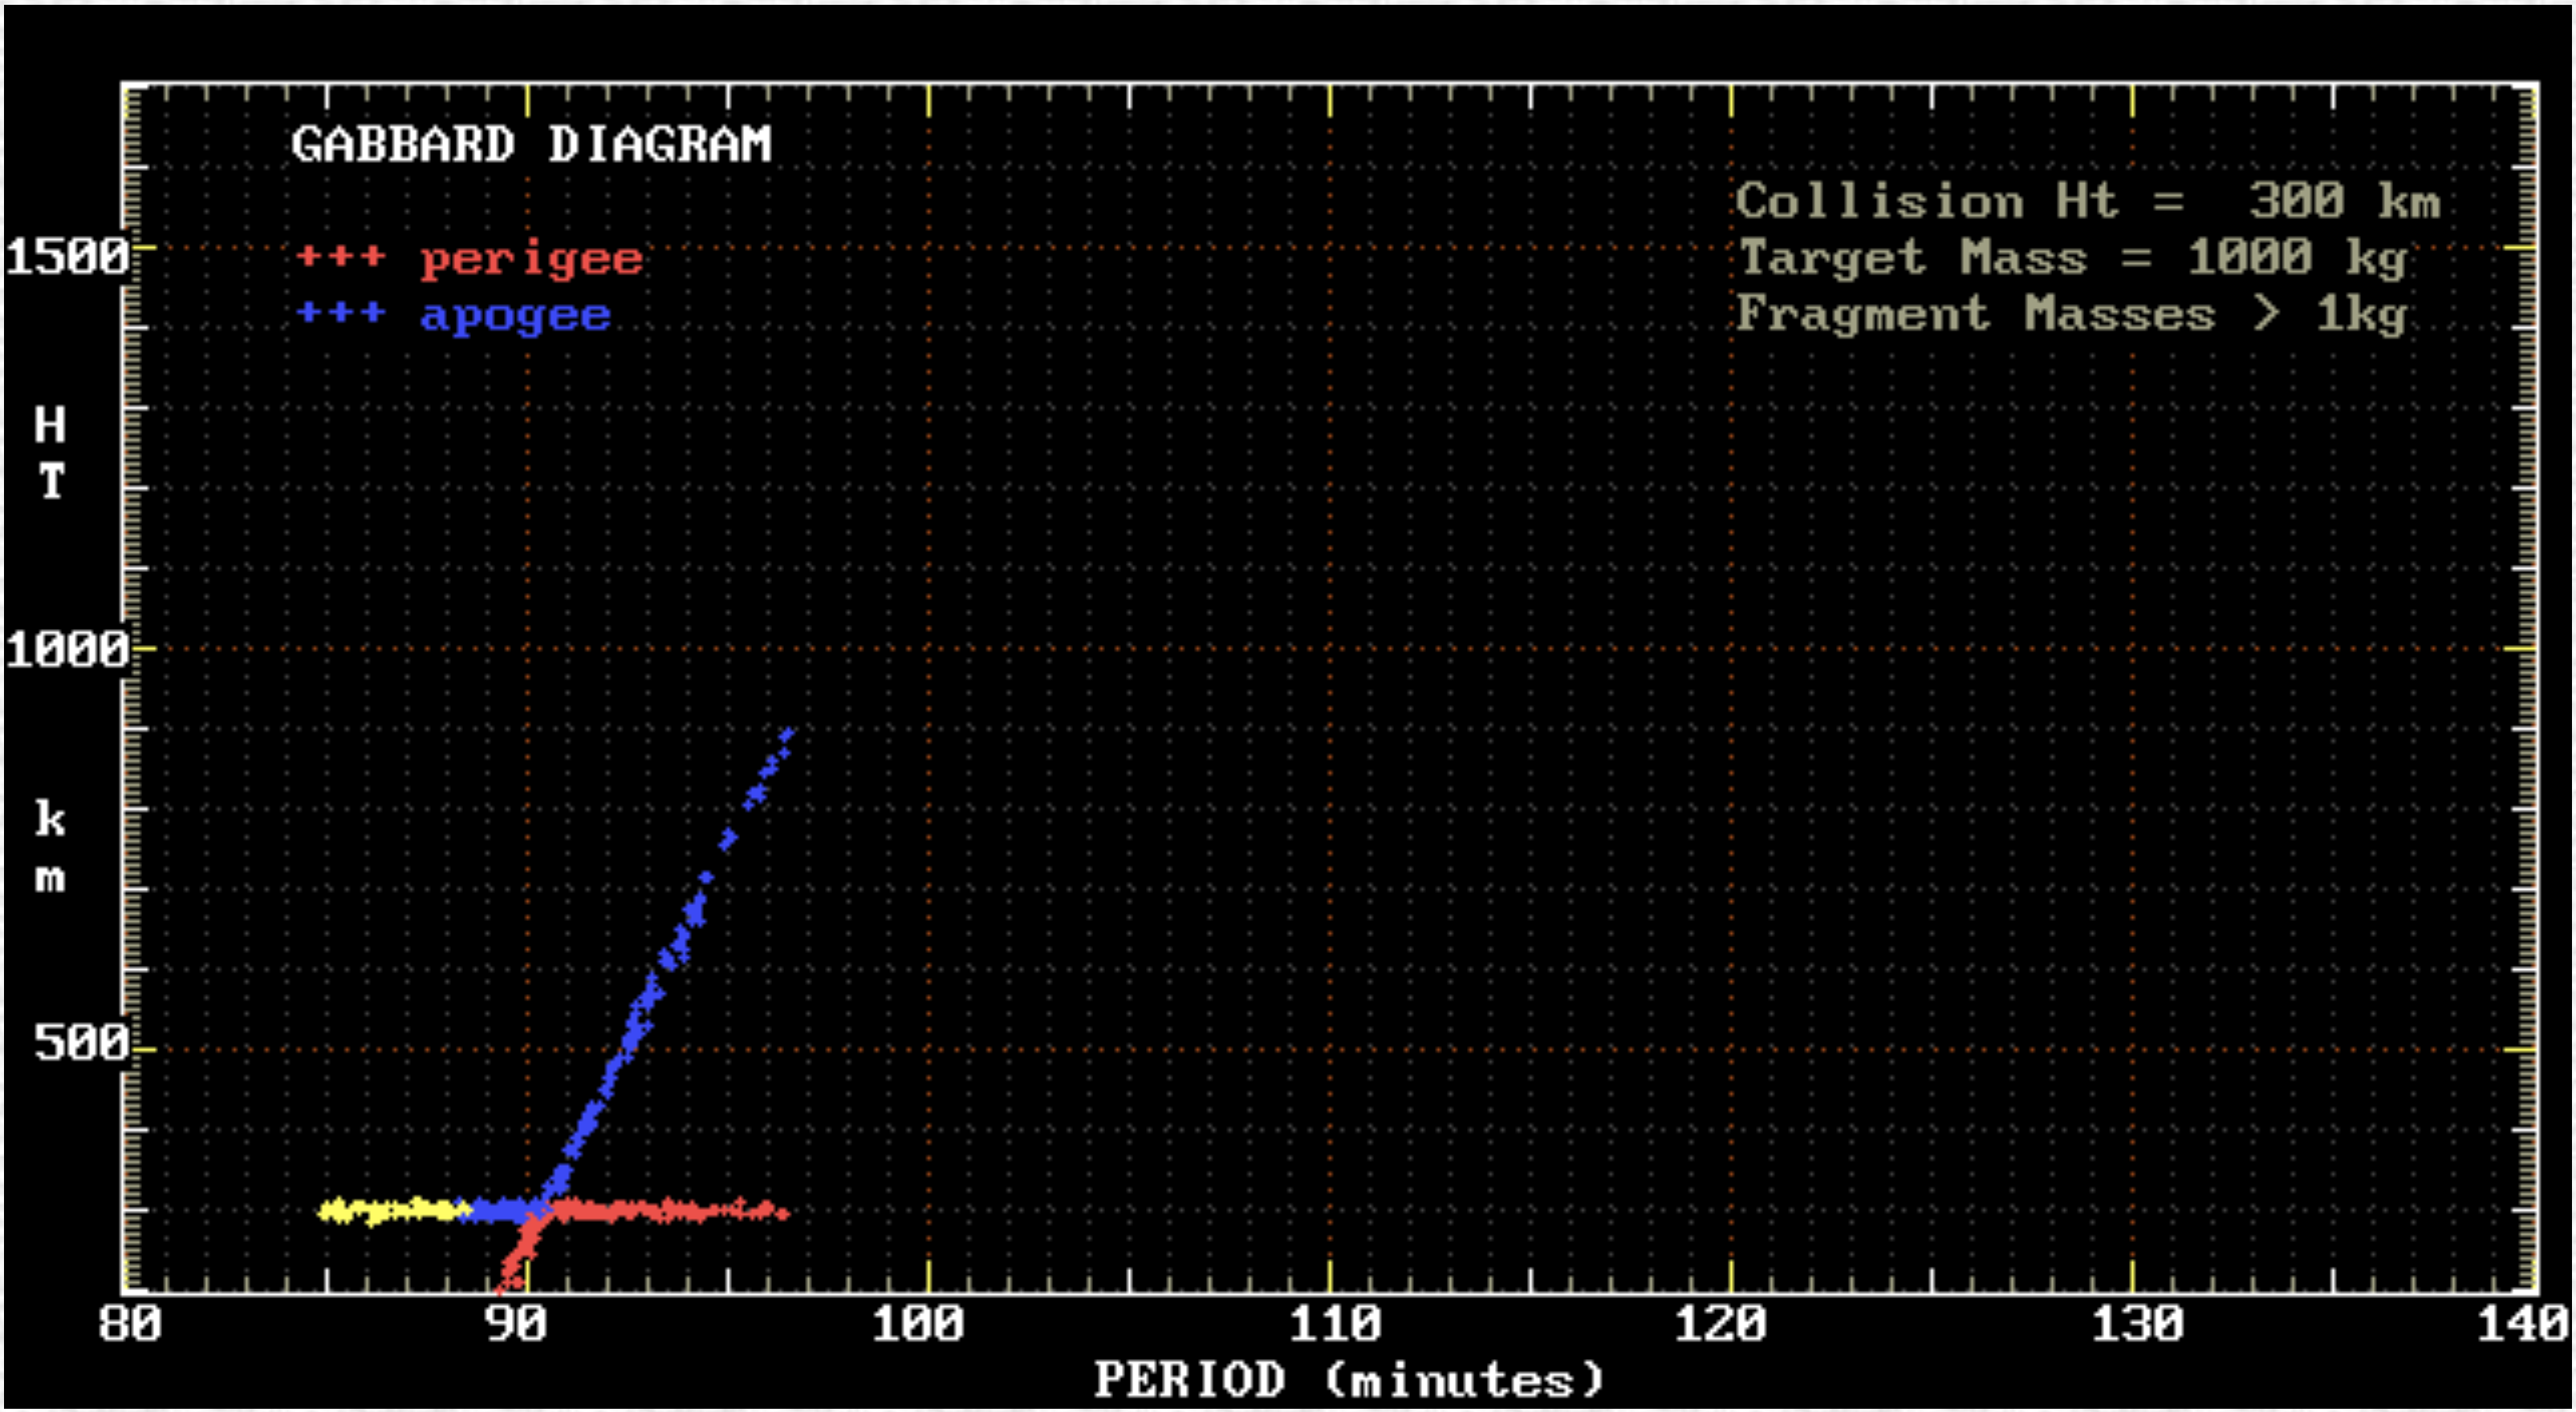
\includegraphics[width=0.8\textwidth]{figure_week_6_gabbard-diagram-decay1-au.png}
    \caption{The yellow points represent fragments with perigees below 100 km, and which are thus not present after one orbit.}
    \label{fig:gabbard-diagram-decay1-au}
  \end{figure}

  \begin{figure}[H]
    \centering
    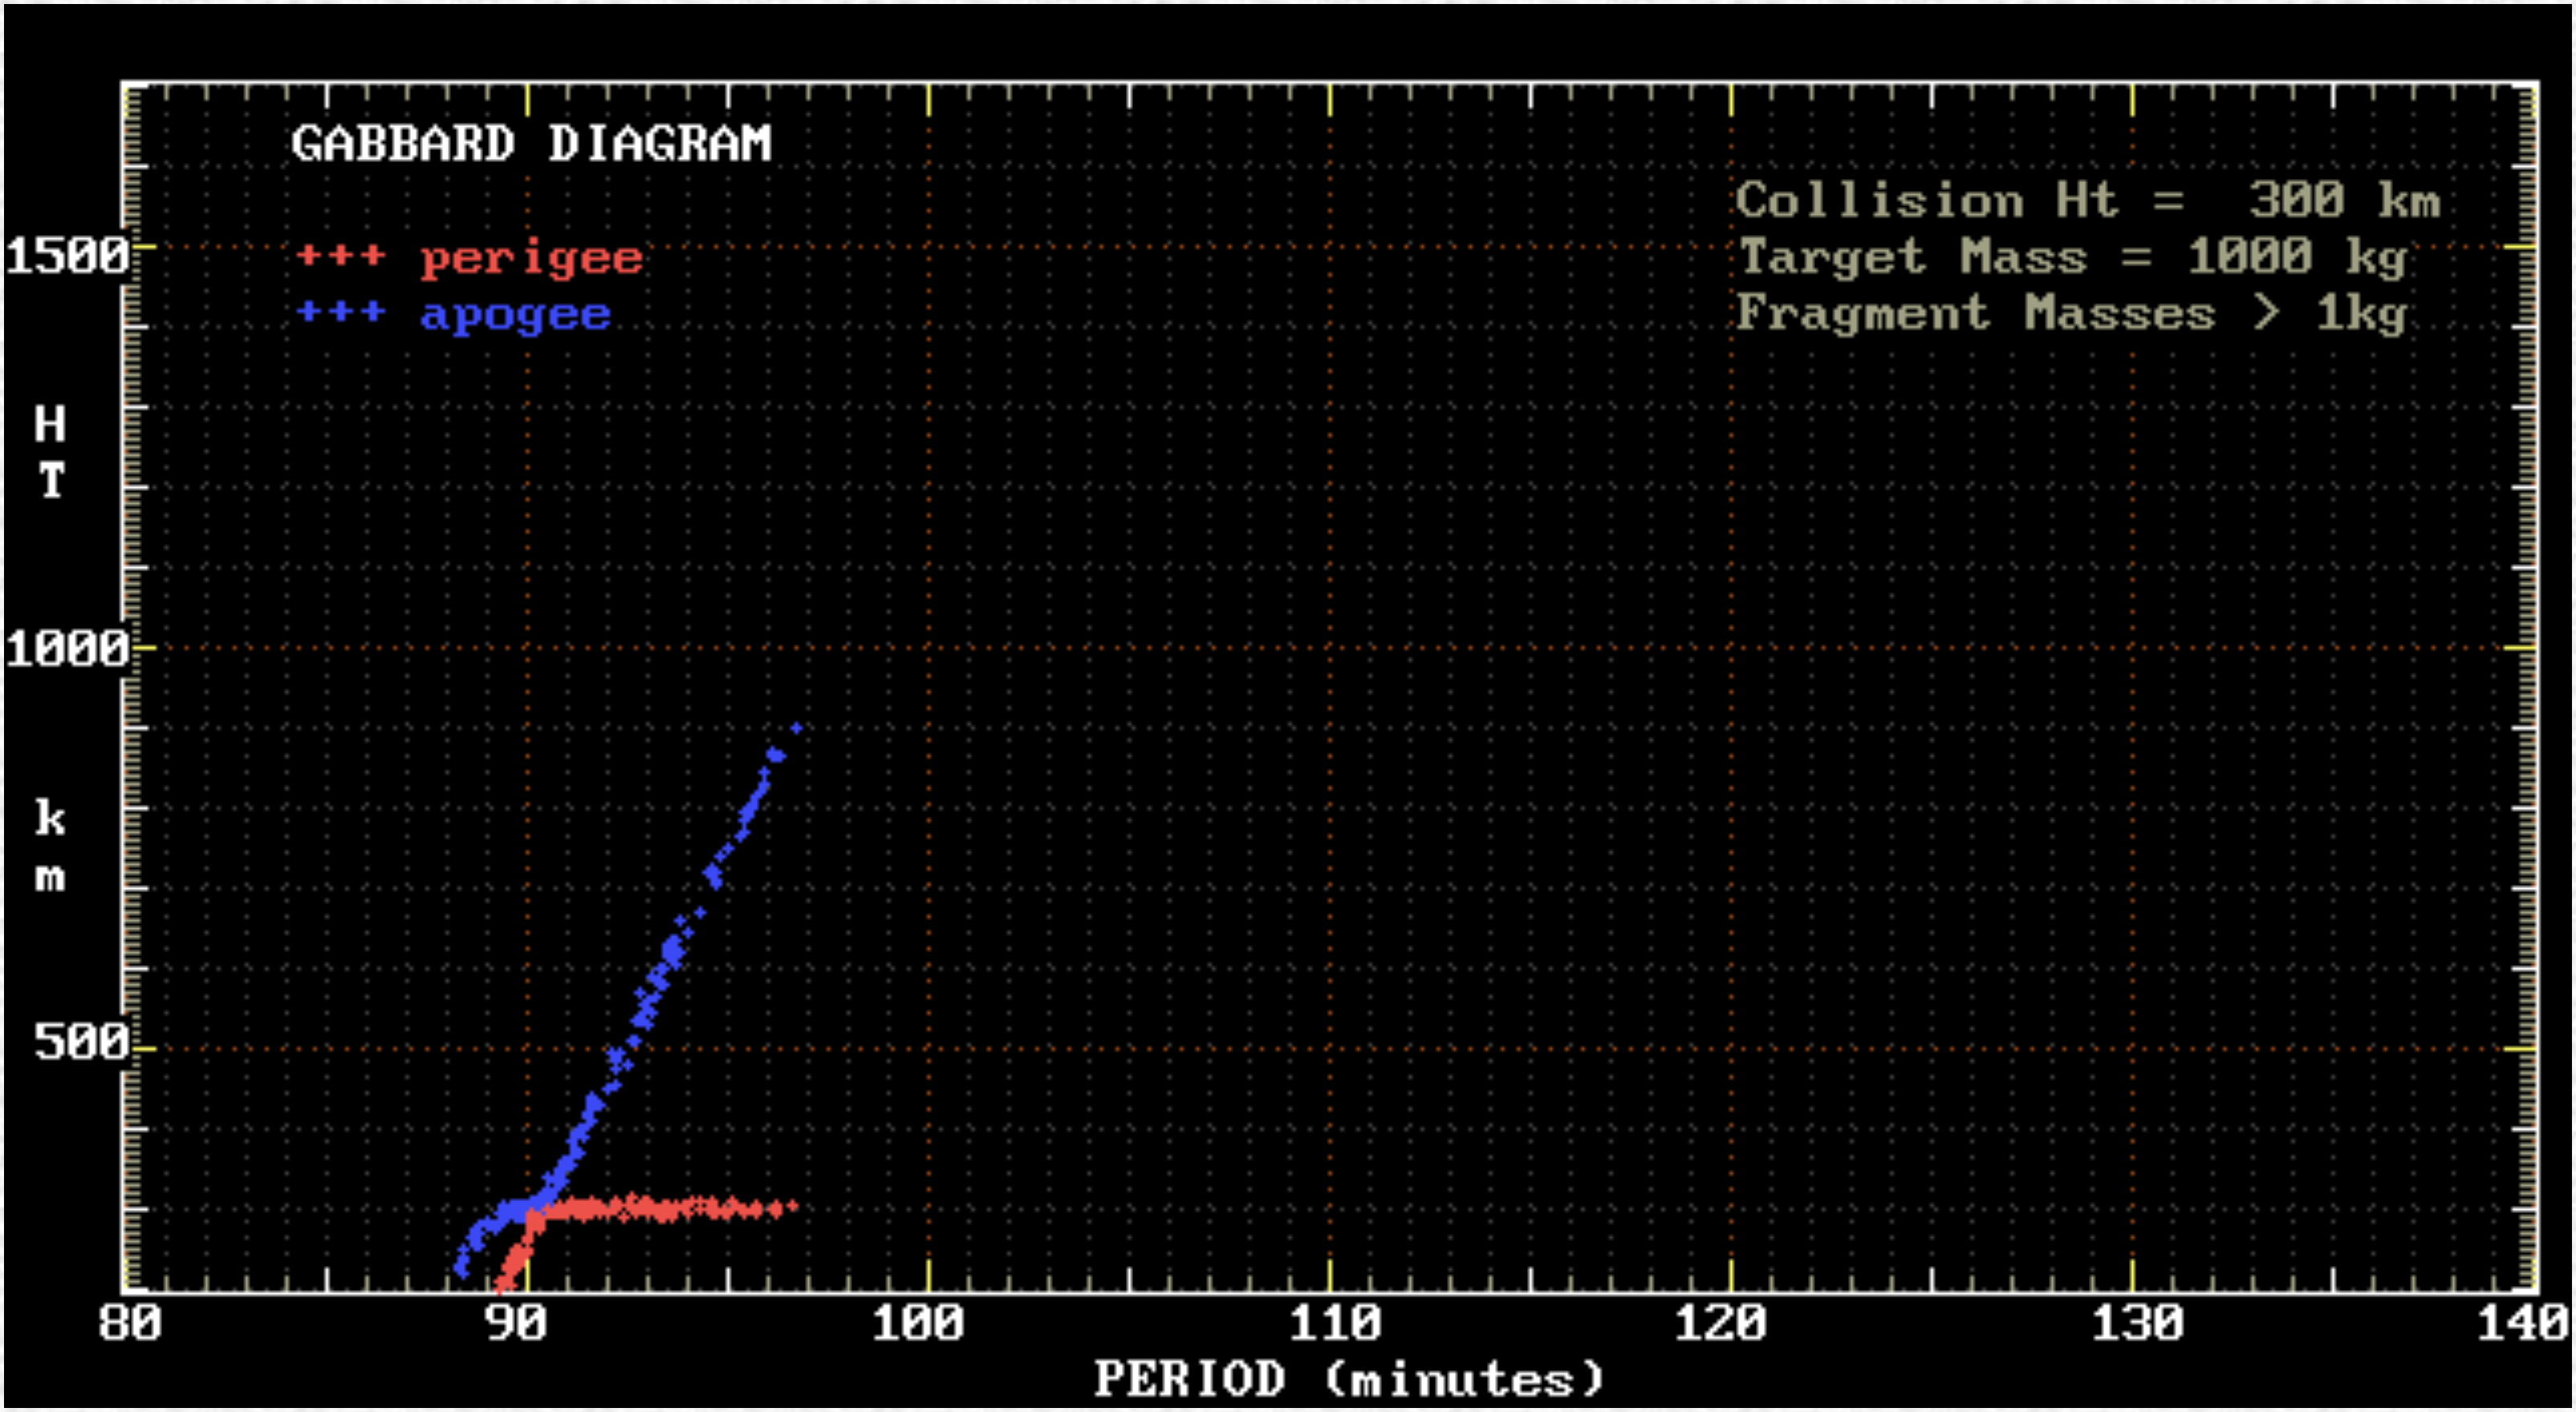
\includegraphics[width=0.8\textwidth]{figure_week_6_gabbard-diagram-decay2-au.png}
    \caption{There is a progressive droop in apogee as the period gets smaller. This plot simulates the fragment population some days after the collision, in conditions of sunspot minimum (i.e. minimal solar X-ray and shortwave UV output, which implies low atmospheric densities in the upper atmosphere).}
    \label{fig:gabbard-diagram-decay2-au}
  \end{figure}

\end{itemize}

\noindent \textbf{Other resources:}
\begin{itemize}
  \item Gabbard Diagram: \url{https://ntrs.nasa.gov/api/citations/20150009502/downloads/20150009502.pdf}
  \item ESA's Hypervelocity Impact Testing: \url{https://www.esa.int/Space_Safety/Space_Debris/Hypervelocity_impacts_and_protecting_spacecraft}
\end{itemize}

\chapter*{Code Changes}

To clean up the code and based on the feedback from Space-Track.org, I decided to make the following changes:

\begin{enumerate}
  
  \item \textbf{My first change was to create two separate scripts for better useability. One script for fetching the TLE data and the other for approach analyisis.}
  
  \begin{figure}[H]
    \centering
    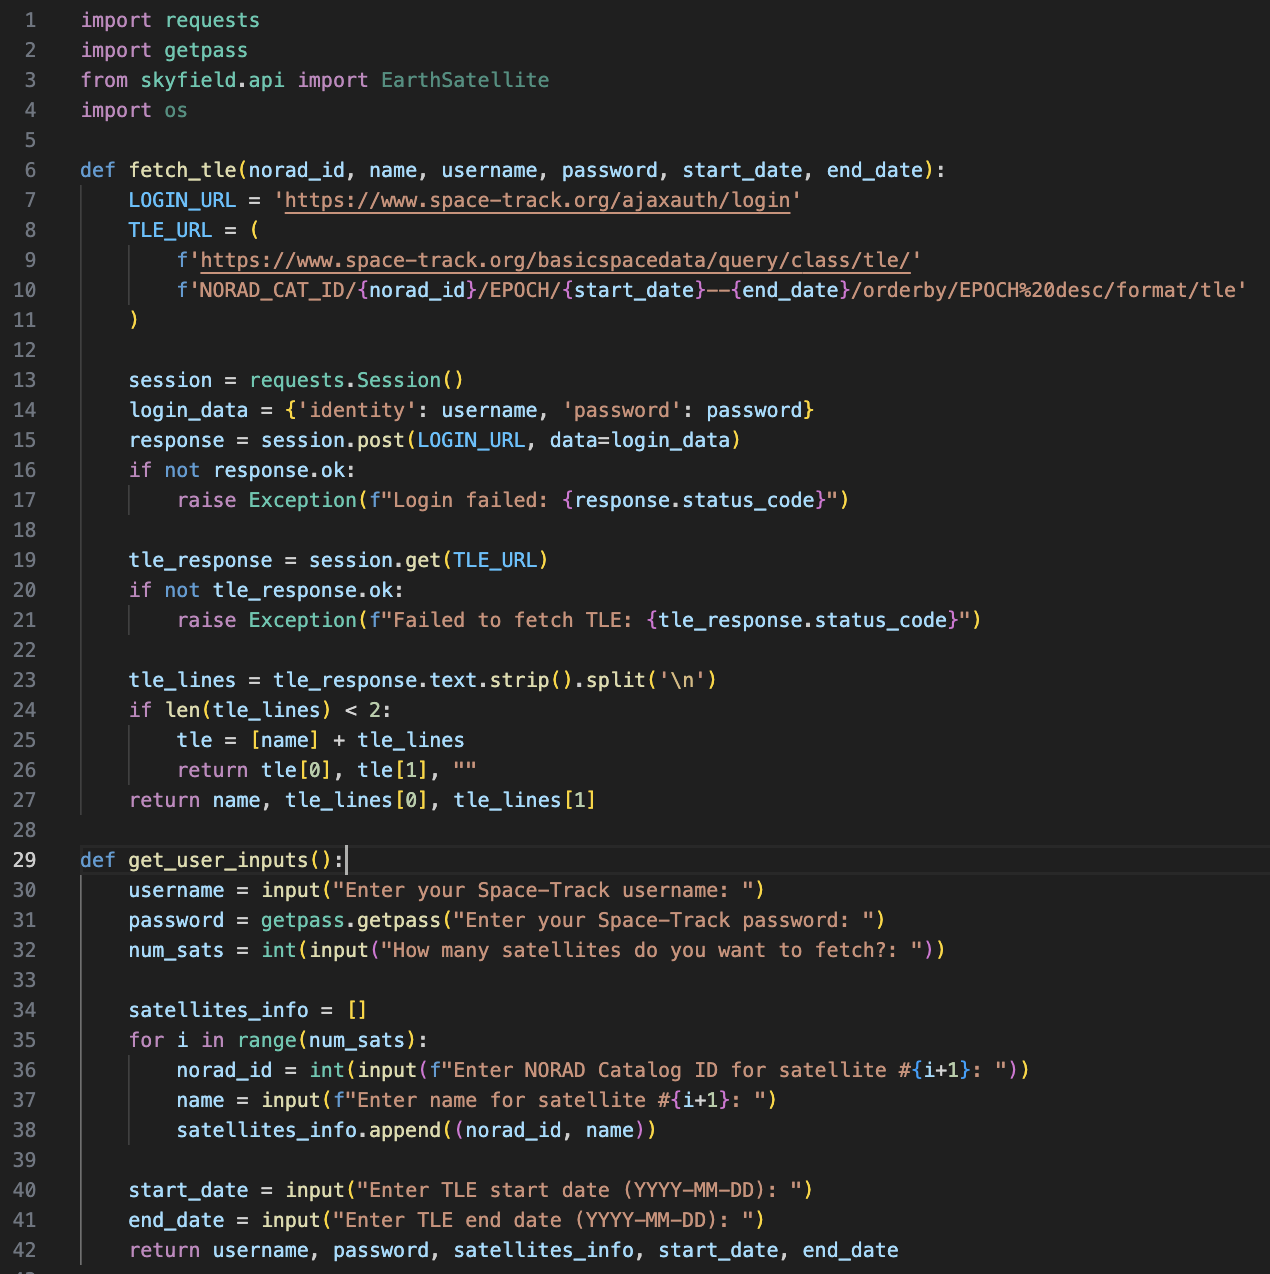
\includegraphics[width=0.8\textwidth]{figure_week_6_fetch-tle-data1.png}
    \caption{Fetching TLE data from Space-Track.org.}
    \label{fig:fetch-tle-data1}
  \end{figure}

  \begin{figure}[H]
    \centering
    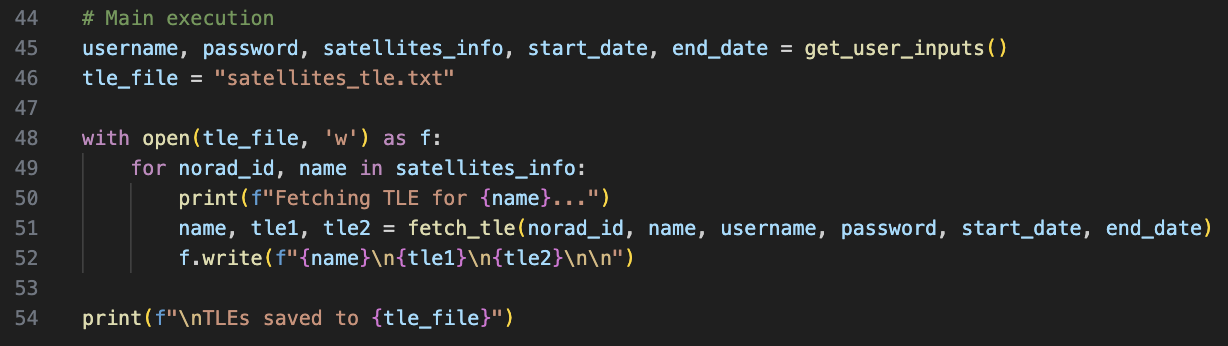
\includegraphics[width=0.8\textwidth]{figure_week_6_fetch-tle-data2.png}
    \caption{Writing the TLE data to a file.}
    \label{fig:analyze-approach}
  \end{figure}

  \begin{figure}[H]
    \centering
    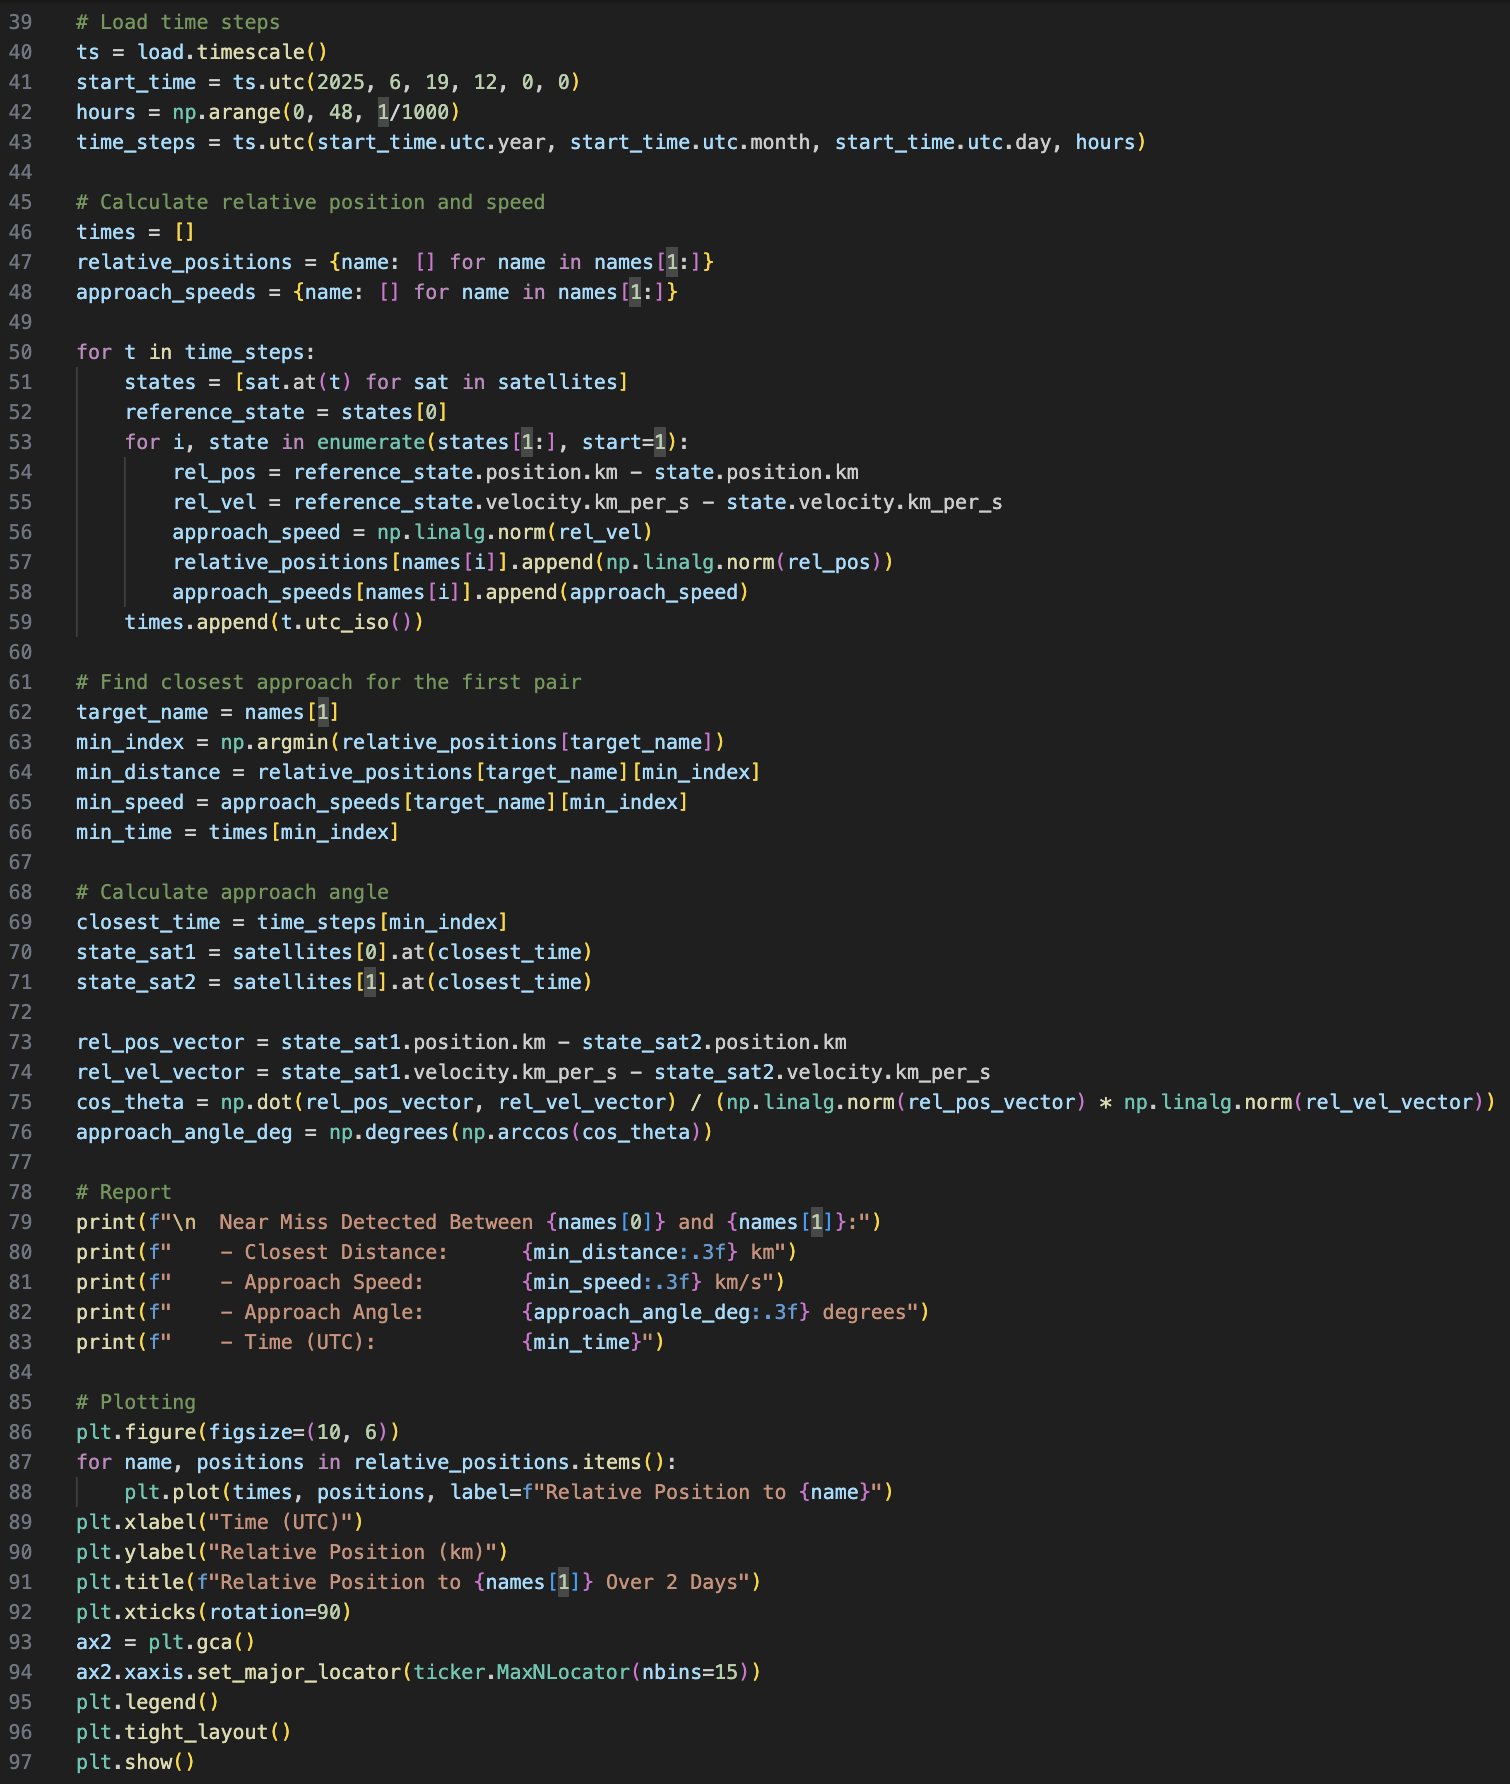
\includegraphics[width=0.8\textwidth]{figure_week_6_analyze-approach.png}
    \caption{Script for analyzing approach conditions.}
    \label{fig:fetch-tle-data2}
  \end{figure}

  \item \textbf{My second change is to make sure that the code does not violate the API rules.}
  
  This was the plan of action that I drafted based on the feedback from Space-Track.org and got approved:
  
  \begin{itemize}
    \item Use of \texttt{/class/gp/} for latest propagable elements: For current TLE data, I will exclusively use: \url{https://www.space-track.org/basicspacedata/query/class/gp/decay_date/null-val/epoch/%3Enow-30/format/tle}.
    \item Avoid deprecated endpoints: I will remove usage of \texttt{/class/tle/}, \texttt{/class/tle\_latest/}, and any other deprecated classes as per Space-Track's notice.
    \item Avoid repeated historical downloads: I will no longer query \texttt{/class/tle/} or \texttt{/class/gp\_history/} multiple times for the same object/date range. Instead, I will download the official yearly zip files from Space-Track's Sync.com archive: \url{https://ln5.sync.com/dl/afd354190/c5cd2q72-a5qjzp4q-nbjdiqkr-cenajuqu}.
    \item No automatic or timed scripts: My current use is manual and academic in nature---the script is not scheduled or automated. However, if I do automate it in the future, I will: Run it 10--20 minutes before or after the hour (i.e., before XX:20 or after XX:40) and/or use batch queries efficiently and responsibly.
  \end{itemize}

  I also got approved for using the Testing URL (strictly for testing):
  \\ \url{https://for-testing-only.space-track.org}
  \\ \\
  API Help Documentation:
  \\ \url{https://for-testing-only.space-track.org/documentation#/api}
  
\end{enumerate}

\chapter*{Next Steps}

\textbf{My Next Steps:}
\begin{itemize}
  \item Research about conjunction analysis, specifically: 
  \begin{itemize}
    \item How do other people propagate orbit to predict collision?
    \item What other parameters are important in conjunction analysis? Propagation techniques, something else other than TLE data?
  \end{itemize}
  \item Implement my plan of action to ensure that the code is compliant with Space-Track's API rules.
  \item Test the new scripts to ensure they work as expected and fetch the latest TLE data correctly. Use the 4 test cases from Week 5 to verify.
\end{itemize}

\noindent \textbf{Dr. Fan's feedback for next steps:}
  \begin{enumerate}
    \item Research what a Gabbard diagram is.
    \item Can I find the spacecraft type (i.e. debris, rocket body, operational satellite) from the TLE data? If so plot data points coresponding to each spacecraft type (by color). The plot can be anything, as long as it can be done.
  \end{enumerate}

\noindent \textbf{End goals:}
\begin{itemize}
  \item Loop through all the TLEs in the LEO category and calculate the approach conditions for each satellite if it is within a certain distance (e.g. 100 km) of the ISS.
  \item Make my code a usable function so Catherine can just call it. Some input \textrightarrow{} Output (approach speed and angle).
\end{itemize}

\end{document}